In this subsection the evaluation of the model trained on ER dataset with stronger regularization is presented. The accuracy of all biological metrics are even better than for nuclei, espesially mean and total intensities correlations are higher. Visually predictions do not look significantly brigher as well. Pearson and Spearman rank correlation coefficients are presented in Table \ref{table:er-downstream-metrics-coefficients}.

\begin{figure}[htb]
	\begin{center}
		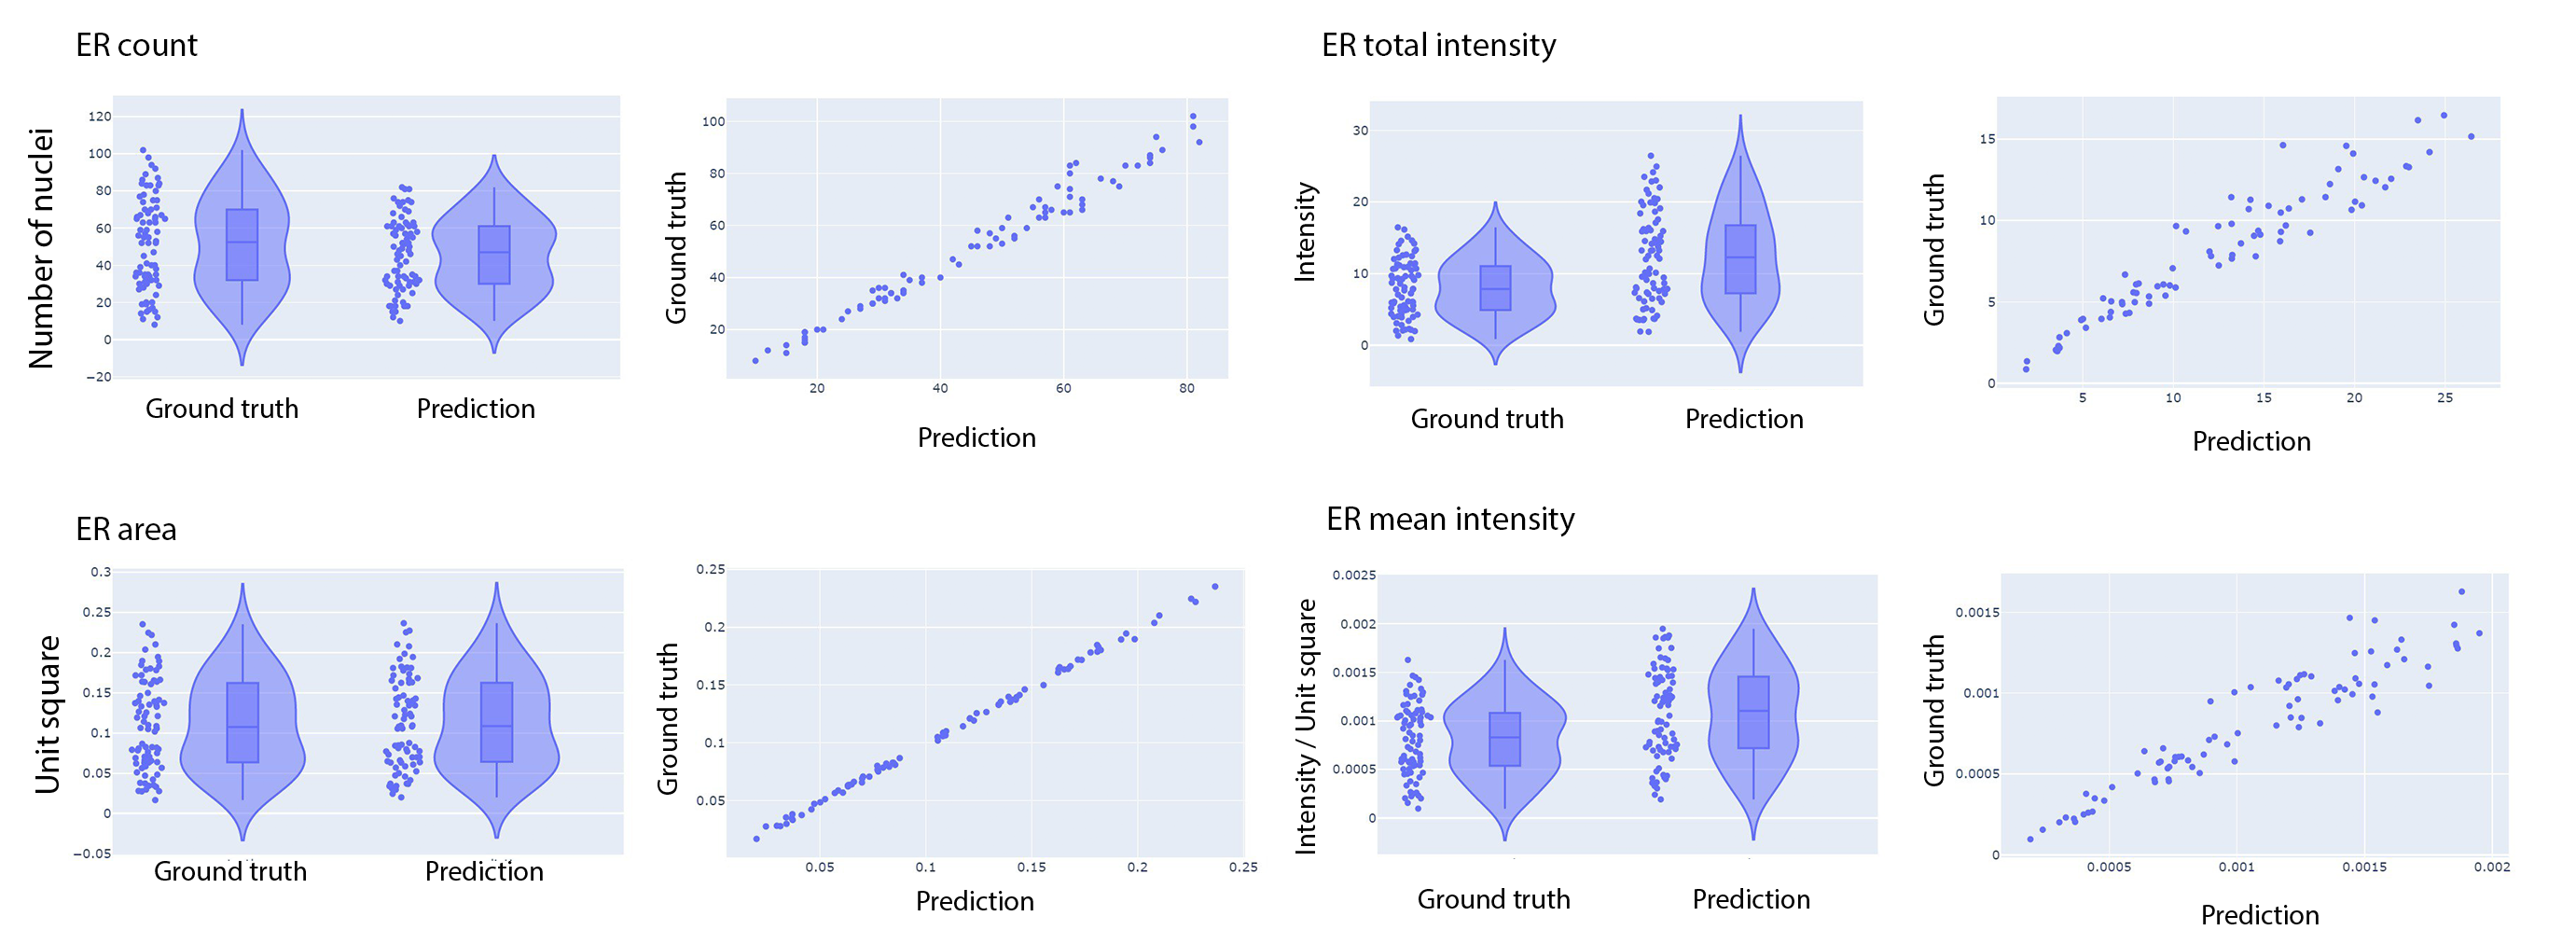
\includegraphics[width=\linewidth]{bilder/ER/metrics/combined-metrics.png}
		\caption{Metrics for biological tasks on ER}\label{fig:er-downstream-metrics}
	\end{center}
\end{figure}

\begin{table}[htb]
    \centering
    \caption{Correlation coefficients for biological tasks on ER}
        \begin{adjustbox}{width=0.4\textwidth}
            \begin{tabular}{|c|c|c|}\hline
                &Pearson&Spearman
                \\\hline\hline
                Number of ER & 0.988 & 0.984\\\hline
                Total intensity&0.952&0.955\\\hline
                Mean intensity&0.941&0.933\\\hline
                Area &0.991&0.990\\\hline
            \end{tabular}
        \label{table:er-downstream-metrics-coefficients}
        \end{adjustbox}
\end{table}
